\documentclass{beamer}
\mode<presentation>
\usepackage{amsmath}
\usepackage{amssymb}
%\usepackage{advdate}
\usepackage{adjustbox}
\usepackage{subcaption}
\usepackage{enumitem}
\usepackage{multicol}
\usepackage{mathtools}
\usepackage{listings}
\usepackage{url}
\def\UrlBreaks{\do\/\do-}
\usetheme{Boadilla}
\usecolortheme{lily}
\setbeamertemplate{footline}
{
  \leavevmode%
  \hbox{%
  \begin{beamercolorbox}[wd=\paperwidth,ht=2.25ex,dp=1ex,right]{author in head/foot}%
    \insertframenumber{} / \inserttotalframenumber\hspace*{2ex} 
  \end{beamercolorbox}}%
  \vskip0pt%
}
\setbeamertemplate{navigation symbols}{}

\providecommand{\nCr}[2]{\,^{#1}C_{#2}} % nCr
\providecommand{\nPr}[2]{\,^{#1}P_{#2}} % nPr
\providecommand{\mbf}{\mathbf}
\providecommand{\pr}[1]{\ensuremath{\Pr\left(#1\right)}}
\providecommand{\qfunc}[1]{\ensuremath{Q\left(#1\right)}}
\providecommand{\sbrak}[1]{\ensuremath{{}\left[#1\right]}}
\providecommand{\lsbrak}[1]{\ensuremath{{}\left[#1\right.}}
\providecommand{\rsbrak}[1]{\ensuremath{{}\left.#1\right]}}
\providecommand{\brak}[1]{\ensuremath{\left(#1\right)}}
\providecommand{\lbrak}[1]{\ensuremath{\left(#1\right.}}
\providecommand{\rbrak}[1]{\ensuremath{\left.#1\right)}}
\providecommand{\cbrak}[1]{\ensuremath{\left\{#1\right\}}}
\providecommand{\lcbrak}[1]{\ensuremath{\left\{#1\right.}}
\providecommand{\rcbrak}[1]{\ensuremath{\left.#1\right\}}}
\theoremstyle{remark}
\newtheorem{rem}{Remark}
\newcommand{\sgn}{\mathop{\mathrm{sgn}}}
\providecommand{\abs}[1]{\left\vert#1\right\vert}
\providecommand{\res}[1]{\Res\displaylimits_{#1}} 
\providecommand{\norm}[1]{\lVert#1\rVert}
\providecommand{\mtx}[1]{\mathbf{#1}}
\providecommand{\mean}[1]{E\left[ #1 \right]}
\providecommand{\fourier}{\overset{\mathcal{F}}{ \rightleftharpoons}}
%\providecommand{\hilbert}{\overset{\mathcal{H}}{ \rightleftharpoons}}
\providecommand{\system}[1]{\overset{\mathcal{#1}}{ \longleftrightarrow}}
%\providecommand{\system}{\overset{\mathcal{H}}{ \longleftrightarrow}}
	%\newcommand{\solution}[2]{\textbf{Solution:}{#1}}
%\newcommand{\solution}{\noindent \textbf{Solution: }}
\providecommand{\dec}[2]{\ensuremath{\overset{#1}{\underset{#2}{\gtrless}}}}
\newcommand{\myvec}[1]{\ensuremath{\begin{pmatrix}#1\end{pmatrix}}}
\let\vec\mathbf

\lstset{
%language=C,
frame=single, 
breaklines=true,
columns=fullflexible
}

\numberwithin{equation}{section}

\title{Signal Processing in High School}
\author{G. V. V. Sharma \\ Dept. of Electrical Engg.,\\IIT Hyderabad.}

\date{\today} 
\begin{document}

\begin{frame}
\titlepage
\end{frame}

\section*{Outline}
\begin{frame}
\tableofcontents
\end{frame}
\section{Two Dice}
\begin{frame}
\frametitle{NCERT}
Two dice, one blue and one grey, are thrown at the same time.   The event defined by the sum of the two numbers appearing on the top of the dice can have 11 possible outcomes 2, 3, 4, 5, 6, 6, 8, 9, 10, 11 and 12.  A student argues that each of these outcomes has a probability $\frac{1}{11}$.  Do you agree with this argument?  Justify your answer.
\end{frame}

\begin{frame}
\frametitle
	{Uniform Distribution: Rectangular Function}
		Let $X_i \in \cbrak{1,2,3,4,5,6}, i = 1,2,$ be the random variables representing the outcome for each die.  Assuming the dice to be fair, the probability mass function (pmf) is expressed as 
\begin{align}
\label{eq:dice_pmf_xi}
p_{X_i}(n) = \pr{X_i = n} = 
\begin{cases}
\frac{1}{6} & 1 \le n \le 6
\\
0 & otherwise
\end{cases}
\end{align}
\end{frame}
\begin{frame}
\frametitle{Sum of Random Variables: Convolution}
\begin{enumerate}[label=\thesection.\arabic*.,ref=\thesection.\theenumi]
	\item The desired outcome is
\begin{align}
\label{eq:dice_xdef}
X &= X_1 + X_2,
\\
\implies X &\in \cbrak{1,2,\dots,12}
\end{align}
%
The objective is to show that
\begin{align}
p_X(n) \ne \frac{1}{11}
\label{eq:dice_wrong}
\end{align}
\item {\em Convolution: }
From \eqref{eq:dice_xdef},
\begin{align}
p_X(n) &= \pr{X_1 + X_2 = n} = \pr{X_1  = n -X_2}
\\
&= \sum_{k}^{}\pr{X_1  = n -k | X_2 = k}p_{X_2}(k)
\label{eq:dice_x_sum}
\end{align}
after unconditioning.  $\because X_1$ and $X_2$ are independent,
\begin{align}
&\pr{X_1  = n -k | X_2 = k} 
	= \pr{X_1  = n -k} = p_{X_1}(n-k)
%\label{eq:dice_x1_indep}
\nonumber \\
\implies
%\end{align}
%From \eqref{eq:dice_x_sum} and \eqref{eq:dice_x1_indep},
%\begin{align}
	&p_X(n) = \sum_{k}^{}p_{X_1}(n-k)p_{X_2}(k) \triangleq p_{X_1}(n)*p_{X_2}(n)
\label{eq:dice_x_conv}
\end{align}
where $*$ denotes the convolution operation. 
\end{enumerate}
\end{frame}
\begin{frame}
\frametitle{Convolution Cont.}
\begin{align}
p_X(n) = \frac{1}{6}\sum_{k=1}^{6}p_{X_1}(n-k)= \frac{1}{6}\sum_{k=n-6}^{n-1}p_{X_1}(k)
\label{eq:dice_x_conv_x1}
\end{align}
\begin{align}
\because p_{X_1}(k) &= 0, \quad k \le 1, k \ge 6.
\end{align}
From \eqref{eq:dice_x_conv_x1},
%
\begin{align}
p_X(n) &= 
\begin{cases}
0 & n < 1
\\
\frac{1}{6}\sum_{k=1}^{n-1}p_{X_1}(k) &  1 \le n-1 \le  6
\\
\frac{1}{6}\sum_{k=n-6}^{6}p_{X_1}(k) & 1 < n-6 \le 6
\\
0 & n > 12
\end{cases}
\label{eq:dice_x_conv_cond}
\end{align}
\end{frame}
\begin{frame}
\frametitle{Triangular Distribution: Student is wrong}
\begin{align}
p_X(n) &= 
\begin{cases}
0 & n < 1
\\
\frac{n-1}{36} &  2 \le n \le  7
\\
\frac{13-n}{36} & 7 < n \le 12
\\
0 & n > 12
\end{cases}
\label{eq:dice_x_conv_final}
\end{align}
\end{frame}
\begin{frame}
\frametitle{Z Transform}
The $Z$-transform of $p_X(n)$ is defined as 
%\cite{proakis_dsp}
\begin{align}
P_X(z) = \sum_{n = -\infty}^{\infty}p_X(n)z^{-n}, \quad z \in \mathbb{C}
\label{eq:dice_xz}
\end{align}
%
From \eqref{eq:dice_pmf_xi} and \eqref{eq:dice_xz}, 
\begin{align}
P_{X_1}(z) =P_{X_2}(z) &= \frac{1}{6}\sum_{n = 1}^{6}z^{-n}
\\
&=\frac{z^{-1}\brak{1-z^{-6}}}{6\brak{1-z^{-1}}}, \quad \abs{z} > 1
\label{eq:dice_xiz}
\end{align}
upon summing up the geometric progression.  
\end{frame}
\begin{frame}
\frametitle{Convolution vs Multiplication}
\begin{align}
p_X(n) &= p_{X_1}(n)*p_{X_2}(n)
\implies
P_X(z) = P_{X_1}(z)P_{X_2}(z)
\label{eq:dice_xzprod_def}
\end{align}
Thus,
\begin{align}
P_X(z) = \cbrak{\frac{z^{-1}\brak{1-z^{-6}}}{6\brak{1-z^{-1}}}}^2
= \frac{1}{36}\frac{z^{-2}\brak{1-2z^{-6}+z^{-12}}}{\brak{1-z^{-1}}^2}
\label{eq:dice_xzprod}
\end{align}
\end{frame}
\begin{frame}
\frametitle{Inverse Z transform}
		The $Z$ transform of $u(n)$ is 
\begin{align}
u(n)&\system{Z} 
 \frac{1}{1-z^{-1}},\,\abs{z} > 1
\end{align}
and
\begin{align}
\label{eq:dice-ramp}
nu(n)&\system{Z} \frac{z^{-1}}{\brak{1-z^{-1}}^2},\,
\abs{z} > 1
\end{align}
\begin{multline}
\frac{1}{36}\sbrak{\brak{n-1}u(n-1) - 2 \brak{n-7}u(n-7)
	+\brak{n-13}u(n-13)}
	\\
\system{Z}
\frac{1}{36}\frac{z^{-2}\brak{1-2z^{-6}+z^{-12}}}{\brak{1-z^{-1}}^2}
\label{eq:dice_xz_closed}
\end{multline}
\end{frame}
\section{Pingala Series}
\begin{frame}
\frametitle{Problem Statement}
Let
\begin{align}
	\label{eq:pingala/10-orig-diff-a}
	a_n &= \frac{\alpha^{n}-\beta^{n}}{\alpha - \beta}, \quad n \ge 1
	\\
	b_n &= a_{n-1} + a_{n+1}, \quad n \ge 2, \quad b_1 =1
	\label{eq:pingala/10-orig-diff}
\end{align}
where $\alpha$ and $\beta$ ($\alpha > \beta$) are the roots of the
\begin{align}
z^2 - z - 1 = 0
\end{align}
%
\end{frame}
\begin{frame}
\frametitle{JEE 2019}
Which of the following options is correct?
\begin{enumerate}[label=\thesection.\arabic*,ref=\thesection.\theenumi]
\item 
	\label{itm:ping-1}
\begin{align}
	\label{eq:ping-1}
	\sum_{k=1}^{n}a_k = a_{n+2}-1, \quad n \ge 1
\end{align}
 \item 
	\label{itm:ping-2}
\begin{align}
	\label{eq:ping-2}
	\sum_{k=1}^{\infty}\frac{a_k}{10^k} =\frac{10}{89}
\end{align}
 \item 
	\label{itm:ping-3}
\begin{align}
	\label{eq:ping-3}
	b_n =\alpha^n + \beta^n, \quad n \ge 1
\end{align}
 \item 
	\label{itm:ping-4}
\begin{align}
	\label{eq:ping-4}
	\sum_{k=1}^{\infty}\frac{b_k}{10^k} =\frac{8}{89}
\end{align}
\end{enumerate}
\end{frame}
\begin{frame}
\frametitle{Difference Equation}
The {\em Pingala} series is generated using the difference equation 
\begin{align}
	x(n+2) = x\brak{n+1} + x\brak{n},  \quad x(0) = x(1) = 1, n \ge 0
	\label{eq:pingala/10-pingala}
\end{align}
\end{frame}
\begin{frame}
\frametitle{One Sided Z transform}
The {\em one sided} $Z$-transform of $x(n)$ is defined as 
\begin{align}
	X^{+}(z) = \sum_{n = 0}^{\infty}x(n)z^{-n}, \quad z \in \mathbb{C}
\label{eq:pingala/one-Z}
\end{align}
Taking the one-sided $Z$-transform on both sides of \eqref{eq:pingala/10-pingala},
\begin{align}
	\mathcal{Z}^+\sbrak{x(n + 2)} &= \mathcal{Z}^+\sbrak{x(n + 1)} + \mathcal{Z}^+\sbrak{x(n)} \\
\implies     z^2X^+(z) - z^2x(0) - zx(1) &= zX^+(z) - zx(0) + zX^+(z) \\
 \implies   \brak{z^2 - z - 1}X^+(z) &= z^2 \\
  \implies    X^+(z) = \frac{1}{1 - z^{-1} - z^{-2}} 
    &= \frac{1}{\brak{1 - \alpha z^{-1}}\brak{1 - \beta z^{-1}}}, \quad |z| > \alpha
    \label{eq:pingala/X-z}
\end{align}
\end{frame}
\begin{frame}
	\frametitle{Inverse}
Expanding $X^+(z)$ in \eqref{eq:pingala/X-z} using partial fractions, we get
\begin{align}
    X^+(z) &= \frac{1}{\brak{\alpha - \beta}}\sbrak{\frac{z}{1 - \alpha z^{-1}} - \frac{z}{1 - \beta z^{-1}}} \\
	\implies    x(n) &= \frac{\alpha^{n + 1} - \beta^{n + 1}}{\alpha - \beta}u(n) 
	\\
	&= a_{n + 1}
    \label{eq:pingala/x-n-def}
\end{align}
upon comparing with
	\eqref{eq:pingala/10-orig-diff-a}.
\end{frame}
\begin{frame}
	\frametitle{Linear Time Invariant System}
	Let 
\begin{align}
	y(n) = x\brak{n-1} + x\brak{n+1},  \quad n \ge 0
	\label{eq:pingala/10-orig-diff-rev}
\end{align}
	Taking the one-sided $Z$-transform on both sides of \eqref{eq:pingala/10-orig-diff-rev},
\begin{align}
	\mathcal{Z}^+\sbrak{y(n)} &= \mathcal{Z}^+\sbrak{x(n + 1)} + \mathcal{Z}^+\sbrak{x(n - 1)} \\
	Y^+(z) &= zX^+(z) - zx(0) + z^{-1}X^+(z) + zx(-1) \\
&= \frac{z + z^{-1}}{1 - z^{-1} - z^{-2}} - z 
= \frac{1 + 2z^{-1}}{1 - z^{-1} - z^{-2}}, \quad |z| > \alpha
\end{align}
\end{frame}
\begin{frame}
	\frametitle{Power of the Z transform}
\begin{align}
	\alpha^n + \beta^n, \quad n \ge 1
    \label{eq:pingala/yn-exp}
\end{align}
can be expressed as 
\begin{align}
	w(n) = \brak{\alpha^{n+1} + \beta^{n+1}}u(n)
\end{align}
Therefore,
\begin{align}
    W(z) = Y(z) = \frac{1 + 2z^{-1}}{1 - z^{-1} - z^{-2}}
\end{align}
\end{frame}
\begin{frame}
\frametitle{Power of the Z transform Cont.}
\begin{align}
    \sum_{k=1}^{\infty}\frac{a_k}{10^k} &= \frac{1}{10}\sum_{k = 0}^{\infty}\frac{a_{k+1}}{10^k} 
                                        = \frac{1}{10}\sum_{k = 0}^{\infty}\frac{x(k)}{10^k} \\
                                        &= \frac{1}{10}X^+(10) 
                                        = \frac{1}{10}\times\frac{100}{89} = \frac{10}{89}
\end{align}
Thus,
\eqref{eq:ping-2} is correct.
\begin{align}
    \sum_{k=1}^{\infty}\frac{b_k}{10^k} &= \frac{1}{10}\sum_{k = 0}^{\infty}\frac{b_{k+1}}{10^k} 
                                        = \frac{1}{10}\sum_{k = 0}^{\infty}\frac{y(k)}{10^k} \\
                                        &= \frac{1}{10}Y^+(z) 
                                        = \frac{1}{10}\times\frac{120}{89} = \frac{12}{89}
\end{align}
Thus,
\eqref{eq:ping-4} is incorrect.
\end{frame}
\begin{frame}
\frametitle{Convolution}
\begin{align}
    \sum_{k=1}^{n}a_k &= \sum_{k=0}^{n-1}x(k) 
                      = \sum_{k = -\infty}^{n - 1}x(k) \\
                      &= \sum_{k = -\infty}^{\infty}x(k)u(n - 1 - k) 
                      = x(n)*u(n - 1)
\end{align}
\begin{align}
a_{n+2}-1, \quad n \ge 1
\end{align}
can be expressed as 
\begin{align}
	\sbrak{x\brak{n+1}-1}u\brak{n-1}
\end{align}
\end{frame}
\begin{frame}
\frametitle{Convolution Cont.}
The Z transform of the above signal can be expressed as
\begin{align}
	\sum_{n = 1}^{\infty}x(n + 1) z^{-n} -\frac{z^{-1}}{1-z^{-1}}
	&=\sum_{n = 2}^{\infty}x(n) z^{-n+1} -\frac{z^{-1}}{1-z^{-1}}
	\\
	&=z\sbrak{X^{+}(z) - x(0) -x(1)z^{-1}} -\frac{z^{-1}}{1-z^{-1}}
	\\
	&= \frac{z}{1 - z^{-1} - z^{-2}} - z - 1 - \frac{z^{-1}}{1 - z^{-1}} \\
	&= \frac{z}{1 - z^{-1} - z^{-2}} -  \frac{z}{1 - z^{-1}} \\
	&=\frac{z^{-1}}{\brak{1 - z^{-1} - z^{-2}}\brak{1 - z^{-1}}} 
\end{align}
From \eqref{eq:pingala/x-n-def}, we get
\begin{align}
    \sum_{k = 1}^{n}a_k = a_{n+2} - 1
\end{align}
\end{frame}
%\iffalse
\documentclass[journal,12pt,twocolumn]{IEEEtran}
%
\usepackage{setspace}
\usepackage{gensymb}
%\doublespacing
\singlespacing

%\usepackage{graphicx}
%\usepackage{amssymb}
%\usepackage{relsize}
\usepackage[cmex10]{amsmath}
\usepackage{siunitx}
%\usepackage{amsthm}
%\interdisplaylinepenalty=2500
%\savesymbol{iint}
%\usepackage{txfonts}
%\restoresymbol{TXF}{iint}
%\usepackage{wasysym}
\usepackage{amsthm}
\usepackage{mathrsfs}
\usepackage{txfonts}
\usepackage{stfloats}
\usepackage{steinmetz}
%\usepackage{bm}
\usepackage{cite}
\usepackage{cases}
\usepackage{subfig}
%\usepackage{xtab}
\usepackage{longtable}
\usepackage{multirow}
%\usepackage{algorithm}
%\usepackage{algpseudocode}
\usepackage{enumitem}
\usepackage{mathtools}
\usepackage{tikz}
\usepackage{circuitikz}
\usepackage{pgfplots}
\usepackage{verbatim}
\usepackage{tfrupee}
\usepackage[breaklinks=true]{hyperref}
%\usepackage{stmaryrd}
\usepackage{tkz-euclide} % loads  TikZ and tkz-base
%\usetkzobj{all}
\usetikzlibrary{calc,math}
\usetikzlibrary{fadings}
\usepackage{listings}
    \usepackage{color}                                            %%
    \usepackage{array}                                            %%
    \usepackage{longtable}                                        %%
    \usepackage{calc}                                             %%
    \usepackage{multirow}                                         %%
    \usepackage{hhline}                                           %%
    \usepackage{ifthen}                                           %%
  %optionally (for landscape tables embedded in another document): %%
    \usepackage{lscape}     
\usepackage{multicol}
\usepackage{chngcntr}
%\usepackage{enumerate}

%\usepackage{wasysym}
%\newcounter{MYtempeqncnt}
\DeclareMathOperator*{\Res}{Res}
%\renewcommand{\baselinestretch}{2}
\renewcommand\thesection{\arabic{section}}
\renewcommand\thesubsection{\thesection.\arabic{subsection}}
\renewcommand\thesubsubsection{\thesubsection.\arabic{subsubsection}}

\renewcommand\thesectiondis{\arabic{section}}
\renewcommand\thesubsectiondis{\thesectiondis.\arabic{subsection}}
\renewcommand\thesubsubsectiondis{\thesubsectiondis.\arabic{subsubsection}}

% correct bad hyphenation here
\hyphenation{op-tical net-works semi-conduc-tor}
\def\inputGnumericTable{}                                 %%

\lstset{
%language=C,
frame=single, 
breaklines=true,
columns=fullflexible
}
%\lstset{
%language=tex,
%frame=single, 
%breaklines=true
%}

\begin{document}
%


\newtheorem{theorem}{Theorem}[section]
\newtheorem{problem}{Problem}
\newtheorem{proposition}{Proposition}[section]
\newtheorem{lemma}{Lemma}[section]
\newtheorem{corollary}[theorem]{Corollary}
\newtheorem{example}{Example}[section]
\newtheorem{definition}[problem]{Definition}
%\newtheorem{thm}{Theorem}[section] 
%\newtheorem{defn}[thm]{Definition}
%\newtheorem{algorithm}{Algorithm}[section]
%\newtheorem{cor}{Corollary}
\newcommand{\BEQA}{\begin{eqnarray}}
\newcommand{\EEQA}{\end{eqnarray}}
\newcommand{\define}{\stackrel{\triangle}{=}}

\bibliographystyle{IEEEtran}
%\bibliographystyle{ieeetr}


\providecommand{\mbf}{\mathbf}
\providecommand{\pr}[1]{\ensuremath{\Pr\left(#1\right)}}
\providecommand{\qfunc}[1]{\ensuremath{Q\left(#1\right)}}
\providecommand{\sbrak}[1]{\ensuremath{{}\left[#1\right]}}
\providecommand{\lsbrak}[1]{\ensuremath{{}\left[#1\right.}}
\providecommand{\rsbrak}[1]{\ensuremath{{}\left.#1\right]}}
\providecommand{\brak}[1]{\ensuremath{\left(#1\right)}}
\providecommand{\lbrak}[1]{\ensuremath{\left(#1\right.}}
\providecommand{\rbrak}[1]{\ensuremath{\left.#1\right)}}
\providecommand{\cbrak}[1]{\ensuremath{\left\{#1\right\}}}
\providecommand{\lcbrak}[1]{\ensuremath{\left\{#1\right.}}
\providecommand{\rcbrak}[1]{\ensuremath{\left.#1\right\}}}
\theoremstyle{remark}
\newtheorem{rem}{Remark}
\newcommand{\sgn}{\mathop{\mathrm{sgn}}}
\providecommand{\abs}[1]{\left\vert#1\right\vert}
\providecommand{\res}[1]{\Res\displaylimits_{#1}} 
\providecommand{\norm}[1]{\left\lVert#1\right\rVert}
%\providecommand{\norm}[1]{\lVert#1\rVert}
\providecommand{\mtx}[1]{\mathbf{#1}}
\providecommand{\mean}[1]{E\left[ #1 \right]}
\providecommand{\fourier}{\overset{\mathcal{F}}{ \rightleftharpoons}}
%\providecommand{\hilbert}{\overset{\mathcal{H}}{ \rightleftharpoons}}
\providecommand{\ztrans}{\overset{\mathcal{Z}}{ \rightleftharpoons}}
\providecommand{\system}{\overset{\mathcal{H}}{ \longleftrightarrow}}
	%\newcommand{\solution}[2]{\textbf{Solution:}{#1}}
\newcommand{\solution}{\noindent \textbf{Solution: }}
\newcommand{\cosec}{\,\text{cosec}\,}
\providecommand{\dec}[2]{\ensuremath{\overset{#1}{\underset{#2}{\gtrless}}}}
\newcommand{\myvec}[1]{\ensuremath{\begin{pmatrix}#1\end{pmatrix}}}
\newcommand{\mydet}[1]{\ensuremath{\begin{vmatrix}#1\end{vmatrix}}}
\providecommand{\gauss}[2]{\mathcal{N}\ensuremath{\left(#1,#2\right)}}
%\providecommand{\system}[1]{\overset{\mathcal{#1}}{ \longleftrightarrow}}
\newcommand*{\permcomb}[4][0mu]{{{}^{#3}\mkern#1#2_{#4}}}
\newcommand*{\perm}[1][-3mu]{\permcomb[#1]{P}}
\newcommand*{\comb}[1][-1mu]{\permcomb[#1]{C}}
%\numberwithin{equation}{section}
\numberwithin{equation}{subsection}
%\numberwithin{problem}{section}
%\numberwithin{definition}{section}
\makeatletter
\@addtoreset{figure}{problem}
\makeatother

\let\StandardTheFigure\thefigure
\let\vec\mathbf
%\renewcommand{\thefigure}{\theproblem.\arabic{figure}}
\renewcommand{\thefigure}{\theproblem}
%\setlist[enumerate,1]{before=\renewcommand\theequation{\theenumi.\arabic{equation}}
%\counterwithin{equation}{enumi}


%\renewcommand{\theequation}{\arabic{subsection}.\arabic{equation}}

\def\putbox#1#2#3{\makebox[0in][l]{\makebox[#1][l]{}\raisebox{\baselineskip}[0in][0in]{\raisebox{#2}[0in][0in]{#3}}}}
     \def\rightbox#1{\makebox[0in][r]{#1}}
     \def\centbox#1{\makebox[0in]{#1}}
     \def\topbox#1{\raisebox{-\baselineskip}[0in][0in]{#1}}
     \def\midbox#1{\raisebox{-0.5\baselineskip}[0in][0in]{#1}}

\vspace{3cm}

\title{
Probability and Random Variables
}
\author{ G V V Sharma$^{*}$% <-this % stops a space
	\thanks{*The author is with the Department
		of Electrical Engineering, Indian Institute of Technology, Hyderabad
		502285 India e-mail:  gadepall@iith.ac.in. All content in this manual is released under GNU GPL.  Free and open source.}
	
}	
%\title{
%	\logo{Matrix Analysis through Octave}{\begin{center}\includegraphics[scale=.24]{tlc}\end{center}}{}{HAMDSP}
%}


% paper title
% can use linebreaks \\ within to get better formatting as desired
%\title{Matrix Analysis through Octave}
%
%
% author names and IEEE memberships
% note positions of commas and nonbreaking spaces ( ~ ) LaTeX will not break
% a structure at a ~ so this keeps an author's name from being broken across
% two lines.
% use \thanks{} to gain access to the first footnote area
% a separate \thanks must be used for each paragraph as LaTeX2e's \thanks
% was not built to handle multiple paragraphs
%

%\author{<-this % stops a space
%\thanks{}}
%}
% note the % following the last \IEEEmembership and also \thanks - 
% these prevent an unwanted space from occurring between the last author name
% and the end of the author line. i.e., if you had this:
% 
% \author{....lastname \thanks{...} \thanks{...} }
%                     ^------------^------------^----Do not want these spaces!
%
% a space would be appended to the last name and could cause every name on that
% line to be shifted left slightly. This is one of those "LaTeX things". For
% instance, "\textbf{A} \textbf{B}" will typeset as "A B" not "AB". To get
% "AB" then you have to do: "\textbf{A}\textbf{B}"
% \thanks is no different in this regard, so shield the last } of each \thanks
% that ends a line with a % and do not let a space in before the next \thanks.
% Spaces after \IEEEmembership other than the last one are OK (and needed) as
% you are supposed to have spaces between the names. For what it is worth,
% this is a minor point as most people would not even notice if the said evil
% space somehow managed to creep in.



% The paper headers
%\markboth{Journal of \LaTeX\ Class Files,~Vol.~6, No.~1, January~2007}%
%{Shell \MakeLowercase{\textit{et al.}}: Bare Demo of IEEEtran.cls for Journals}
% The only time the second header will appear is for the odd numbered pages
% after the title page when using the twoside option.
% 
% *** Note that you probably will NOT want to include the author's ***
% *** name in the headers of peer review papers.                   ***
% You can use \ifCLASSOPTIONpeerreview for conditional compilation here if
% you desire.




% If you want to put a publisher's ID mark on the page you can do it like
% this:
%\IEEEpubid{0000--0000/00\$00.00~\copyright~2007 IEEE}
% Remember, if you use this you must call \IEEEpubidadjcol in the second
% column for its text to clear the IEEEpubid mark.



% make the title area
\maketitle

\newpage

\tableofcontents

\bigskip

\renewcommand{\thefigure}{\theenumi}
\renewcommand{\thetable}{\theenumi}
%\renewcommand{\theequation}{\theenumi}

%\begin{abstract}
%%\boldmath
%In this letter, an algorithm for evaluating the exact analytical bit error rate  (BER)  for the piecewise linear (PL) combiner for  multiple relays is presented. Previous results were available only for upto three relays. The algorithm is unique in the sense that  the actual mathematical expressions, that are prohibitively large, need not be explicitly obtained. The diversity gain due to multiple relays is shown through plots of the analytical BER, well supported by simulations. 
%
%\end{abstract}
% IEEEtran.cls defaults to using nonbold math in the Abstract.
% This preserves the distinction between vectors and scalars. However,
% if the journal you are submitting to favors bold math in the abstract,
% then you can use LaTeX's standard command \boldmath at the very start
% of the abstract to achieve this. Many IEEE journals frown on math
% in the abstract anyway.

% Note that keywords are not normally used for peerreview papers.
%\begin{IEEEkeywords}
%Cooperative diversity, decode and forward, piecewise linear
%\end{IEEEkeywords}



% For peer review papers, you can put extra information on the cover
% page as needed:
% \ifCLASSOPTIONpeerreview
% \begin{center} \bfseries EDICS Category: 3-BBND \end{center}
% \fi
%
% For peerreview papers, this IEEEtran command inserts a page break and
% creates the second title. It will be ignored for other modes.
%\IEEEpeerreviewmaketitle

%\begin{abstract}
%This book provides a simple introduction to probability and random variables.   The contents are largely based on  NCERT textbooks from Class 9-12.
%\end{abstract}


%\section{Axioms of Probability}
%\input{./chapters/axioms.tex}
\fi

\section{Sum of Independent Random Variables}
Two dice, one blue and one grey, are thrown at the same time.   The event defined by the sum of the two numbers appearing on the top of the dice can have 11 possible outcomes 2, 3, 4, 5, 6, 6, 8, 9, 10, 11 and 12.  A student argues that each of these outcomes has a probability $\frac{1}{11}$.  Do you agree with this argument?  Justify your answer.

\renewcommand{\theequation}{\theenumi}
\renewcommand{\thefigure}{\theenumi}
\begin{enumerate}[label=\thesection.\arabic*.,ref=\thesection.\theenumi]
\numberwithin{equation}{enumi}
\numberwithin{figure}{enumi}

%

\item  {\em The Uniform Distribution: }Let $X_i \in \cbrak{1,2,3,4,5,6}, i = 1,2,$ be the random variables representing the outcome for each die.  Assuming the dice to be fair, the probability mass function (pmf) is expressed as 
\begin{align}
\label{eq:dice_pmf_xi}
p_{X_i}(n) = \pr{X_i = n} = 
\begin{cases}
\frac{1}{6} & 1 \le n \le 6
\\
0 & otherwise
\end{cases}
\end{align}
The desired outcome is
\begin{align}
\label{eq:dice_xdef}
X &= X_1 + X_2,
\\
\implies X &\in \cbrak{1,2,\dots,12}
\end{align}
%
The objective is to show that
\begin{align}
p_X(n) \ne \frac{1}{11}
\label{eq:dice_wrong}
\end{align}
\item {\em Convolution: }
From \eqref{eq:dice_xdef},
\begin{align}
p_X(n) &= \pr{X_1 + X_2 = n} = \pr{X_1  = n -X_2}
\\
&= \sum_{k}^{}\pr{X_1  = n -k | X_2 = k}p_{X_2}(k)
\label{eq:dice_x_sum}
\end{align}
after unconditioning.  $\because X_1$ and $X_2$ are independent,
\begin{multline}
\pr{X_1  = n -k | X_2 = k} 
\\
= \pr{X_1  = n -k} = p_{X_1}(n-k)
\label{eq:dice_x1_indep}
\end{multline}
From \eqref{eq:dice_x_sum} and \eqref{eq:dice_x1_indep},
\begin{align}
p_X(n) = \sum_{k}^{}p_{X_1}(n-k)p_{X_2}(k) = p_{X_1}(n)*p_{X_2}(n)
\label{eq:dice_x_conv}
\end{align}
where $*$ denotes the convolution operation. 
%\cite{proakis_dsp}.  
Substituting from \eqref{eq:dice_pmf_xi}
in \eqref{eq:dice_x_conv},
\begin{align}
p_X(n) = \frac{1}{6}\sum_{k=1}^{6}p_{X_1}(n-k)= \frac{1}{6}\sum_{k=n-6}^{n-1}p_{X_1}(k)
\label{eq:dice_x_conv_x1}
\end{align}
\begin{align}
\because p_{X_1}(k) &= 0, \quad k \le 1, k \ge 6.
\end{align}
From \eqref{eq:dice_x_conv_x1},
%
\begin{align}
p_X(n) &= 
\begin{cases}
0 & n < 1
\\
\frac{1}{6}\sum_{k=1}^{n-1}p_{X_1}(k) &  1 \le n-1 \le  6
\\
\frac{1}{6}\sum_{k=n-6}^{6}p_{X_1}(k) & 1 < n-6 \le 6
\\
0 & n > 12
\end{cases}
\label{eq:dice_x_conv_cond}
\end{align}
Substituting from \eqref{eq:dice_pmf_xi} in \eqref{eq:dice_x_conv_cond},
\begin{align}
p_X(n) &= 
\begin{cases}
0 & n < 1
\\
\frac{n-1}{36} &  2 \le n \le  7
\\
\frac{13-n}{36} & 7 < n \le 12
\\
0 & n > 12
\end{cases}
\label{eq:dice_x_conv_final}
\end{align}
satisfying \eqref{eq:dice_wrong}.
\item {\em The $Z$-transform: }
The $Z$-transform of $p_X(n)$ is defined as 
%\cite{proakis_dsp}
\begin{align}
P_X(z) = \sum_{n = -\infty}^{\infty}p_X(n)z^{-n}, \quad z \in \mathbb{C}
\label{eq:dice_xz}
\end{align}
%
From \eqref{eq:dice_pmf_xi} and \eqref{eq:dice_xz}, 
\begin{align}
P_{X_1}(z) =P_{X_2}(z) &= \frac{1}{6}\sum_{n = 1}^{6}z^{-n}
\\
&=\frac{z^{-1}\brak{1-z^{-6}}}{6\brak{1-z^{-1}}}, \quad \abs{z} > 1
\label{eq:dice_xiz}
\end{align}
upon summing up the geometric progression.  
\begin{align}
\because p_X(n) &= p_{X_1}(n)*p_{X_2}(n),
\\
P_X(z) &= P_{X_1}(z)P_{X_2}(z)
\label{eq:dice_xzprod_def}
\end{align}
The above property follows from Fourier analysis and is fundamental to signal processing. 
%\cite{proakis_dsp}. 
From \eqref{eq:dice_xiz} and \eqref{eq:dice_xzprod_def},
\begin{align}
P_X(z) &= \cbrak{\frac{z^{-1}\brak{1-z^{-6}}}{6\brak{1-z^{-1}}}}^2
\\
&= \frac{1}{36}\frac{z^{-2}\brak{1-2z^{-6}+z^{-12}}}{\brak{1-z^{-1}}^2}
\label{eq:dice_xzprod}
\end{align}
Using the fact that 
%\cite{proakis_dsp}
\begin{align}
p_X(n-k) &\system{Z}P_X(z)z^{-k},
\\
nu(n)&\system{Z} \frac{z^{-1}}{\brak{1-z^{-1}}^2}
\end{align}
after some algebra, it can be shown that
%{\tiny
\begin{multline}
\frac{1}{36}\lsbrak{\brak{n-1}u(n-1) - 2 \brak{n-7}u(n-7)}
\\
\rsbrak{ +\brak{n-13}u(n-13)}
\\
\system{Z}
\frac{1}{36}\frac{z^{-2}\brak{1-2z^{-6}+z^{-12}}}{\brak{1-z^{-1}}^2}
\label{eq:dice_xz_closed}
\end{multline}
%}

where 
\begin{align}
u(n) =
\begin{cases}
1 & n \ge 0
\\
0 & n < 0
\end{cases}
\end{align}

From \eqref{eq:dice_xz}, \eqref{eq:dice_xzprod} and \eqref{eq:dice_xz_closed}
\begin{multline}
p_{X}(n) = \frac{1}{36}\lsbrak{\brak{n-1}u(n-1) 
}
\\
\rsbrak{- 2 \brak{n-7}u(n-7)+\brak{n-13}u(n-13)}
\end{multline}
which is the same as \eqref{eq:dice_x_conv_final}.  Note that  \eqref{eq:dice_x_conv_final} can be obtained from \eqref{eq:dice_xz_closed} using contour integration as well.
% \cite{proakis_dsp}.  

\item 
The experiment of rolling the dice was simulated using Python for 10000 samples.  These were generated using Python libraries for uniform distribution. The frequencies for each outcome were then used to compute the resulting pmf, which  is plotted in Figure \ref{fig:dice}.  The theoretical pmf obtained in \eqref{eq:dice_x_conv_final} is plotted for comparison.  
%
\begin{figure}[!ht]
\centering
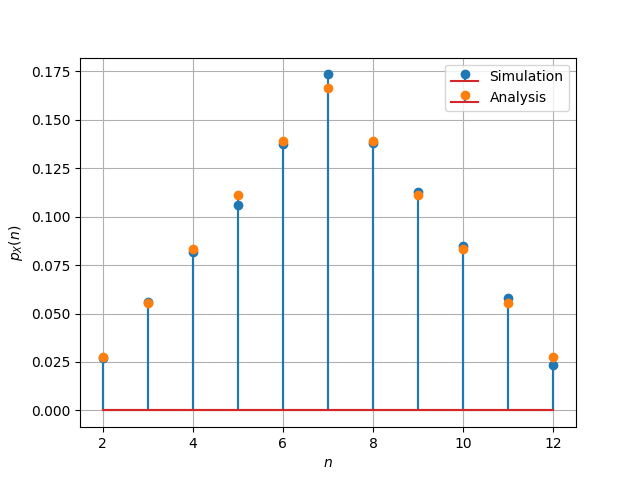
\includegraphics[width=\columnwidth]{./conv-trans/figs/sum/pmf.png}
\caption{Plot of $p_X(n)$.  Simulations are close to the analysis. }
\label{fig:dice}
\end{figure}
\item The python code is available in 
\begin{lstlisting}
/codes/sum/dice.py
\end{lstlisting}

%\item 
%We have shown how a simple problem of throwing a dice can be used for learning not just probability but concepts in  signal processing as well.  Inversion of the $Z$-transform for finding the pmf using contour integration, though not discussed here, opens a window to complex analysis too.  Note that the solutions that are provided  can be easily understood using high school math like arithmetic and geometric sums.  Thus, school students can use a bit of college level math to obtain simpler solutions to their problems.  College students can be exposed to advanced mathematics through simple problems from high school texts.  In addition, both can learn how to verify theoretical results through computer simulations.

%\bibliographystyle{tMES}
%\bibliography{school}
%
%\end{document}
\end{enumerate}
%\subsection{The Uniform Distribution}
%\input{./chapters/sum.tex}
%\section{Cumulative Distribution Function}
%\subsection{The Bernoulli Distribution}
%%%%%%%%%%%%%%%%%%%%%%%%%%%%%%%%%%%%%%%%%%%%%%%%%%%%%%%%%%%%%%%%%%%%%%%
%%                                                                  %%
%%  This is the header of a LaTeX2e file exported from Gnumeric.    %%
%%                                                                  %%
%%  This file can be compiled as it stands or included in another   %%
%%  LaTeX document. The table is based on the longtable package so  %%
%%  the longtable options (headers, footers...) can be set in the   %%
%%  preamble section below (see PRAMBLE).                           %%
%%                                                                  %%
%%  To include the file in another, the following two lines must be %%
%%  in the including file:                                          %%
%%        \def\inputGnumericTable{}                                 %%
%%  at the beginning of the file and:                               %%
%%        \input{name-of-this-file.tex}                             %%
%%  where the table is to be placed. Note also that the including   %%
%%  file must use the following packages for the table to be        %%
%%  rendered correctly:                                             %%
%%    \usepackage[latin1]{inputenc}                                 %%
%%    \usepackage{color}                                            %%
%%    \usepackage{array}                                            %%
%%    \usepackage{longtable}                                        %%
%%    \usepackage{calc}                                             %%
%%    \usepackage{multirow}                                         %%
%%    \usepackage{hhline}                                           %%
%%    \usepackage{ifthen}                                           %%
%%  optionally (for landscape tables embedded in another document): %%
%%    \usepackage{lscape}                                           %%
%%                                                                  %%
%%%%%%%%%%%%%%%%%%%%%%%%%%%%%%%%%%%%%%%%%%%%%%%%%%%%%%%%%%%%%%%%%%%%%%



%%  This section checks if we are begin input into another file or  %%
%%  the file will be compiled alone. First use a macro taken from   %%
%%  the TeXbook ex 7.7 (suggestion of Han-Wen Nienhuys).            %%
\def\ifundefined#1{\expandafter\ifx\csname#1\endcsname\relax}


%%  Check for the \def token for inputed files. If it is not        %%
%%  defined, the file will be processed as a standalone and the     %%
%%  preamble will be used.                                          %%
\ifundefined{inputGnumericTable}

%%  We must be able to close or not the document at the end.        %%
	\def\gnumericTableEnd{\end{document}}


%%%%%%%%%%%%%%%%%%%%%%%%%%%%%%%%%%%%%%%%%%%%%%%%%%%%%%%%%%%%%%%%%%%%%%
%%                                                                  %%
%%  This is the PREAMBLE. Change these values to get the right      %%
%%  paper size and other niceties.                                  %%
%%                                                                  %%
%%%%%%%%%%%%%%%%%%%%%%%%%%%%%%%%%%%%%%%%%%%%%%%%%%%%%%%%%%%%%%%%%%%%%%

	\documentclass[12pt%
			  %,landscape%
                    ]{report}
       \usepackage[latin1]{inputenc}
       \usepackage{fullpage}
       \usepackage{color}
       \usepackage{array}
       \usepackage{longtable}
       \usepackage{calc}
       \usepackage{multirow}
       \usepackage{hhline}
       \usepackage{ifthen}

	\begin{document}


%%  End of the preamble for the standalone. The next section is for %%
%%  documents which are included into other LaTeX2e files.          %%
\else

%%  We are not a stand alone document. For a regular table, we will %%
%%  have no preamble and only define the closing to mean nothing.   %%
    \def\gnumericTableEnd{}

%%  If we want landscape mode in an embedded document, comment out  %%
%%  the line above and uncomment the two below. The table will      %%
%%  begin on a new page and run in landscape mode.                  %%
%       \def\gnumericTableEnd{\end{landscape}}
%       \begin{landscape}


%%  End of the else clause for this file being \input.              %%
\fi

%%%%%%%%%%%%%%%%%%%%%%%%%%%%%%%%%%%%%%%%%%%%%%%%%%%%%%%%%%%%%%%%%%%%%%
%%                                                                  %%
%%  The rest is the gnumeric table, except for the closing          %%
%%  statement. Changes below will alter the table's appearance.     %%
%%                                                                  %%
%%%%%%%%%%%%%%%%%%%%%%%%%%%%%%%%%%%%%%%%%%%%%%%%%%%%%%%%%%%%%%%%%%%%%%

\providecommand{\gnumericmathit}[1]{#1} 
%%  Uncomment the next line if you would like your numbers to be in %%
%%  italics if they are italizised in the gnumeric table.           %%
%\renewcommand{\gnumericmathit}[1]{\mathit{#1}}
\providecommand{\gnumericPB}[1]%
{\let\gnumericTemp=\\#1\let\\=\gnumericTemp\hspace{0pt}}
 \ifundefined{gnumericTableWidthDefined}
        \newlength{\gnumericTableWidth}
        \newlength{\gnumericTableWidthComplete}
        \newlength{\gnumericMultiRowLength}
        \global\def\gnumericTableWidthDefined{}
 \fi
%% The following setting protects this code from babel shorthands.  %%
 \ifthenelse{\isundefined{\languageshorthands}}{}{\languageshorthands{english}}
%%  The default table format retains the relative column widths of  %%
%%  gnumeric. They can easily be changed to c, r or l. In that case %%
%%  you may want to comment out the next line and uncomment the one %%
%%  thereafter                                                      %%
\providecommand\gnumbox{\makebox[0pt]}
%%\providecommand\gnumbox[1][]{\makebox}

%% to adjust positions in multirow situations                       %%
\setlength{\bigstrutjot}{\jot}
\setlength{\extrarowheight}{\doublerulesep}

%%  The \setlongtables command keeps column widths the same across  %%
%%  pages. Simply comment out next line for varying column widths.  %%
\setlongtables

\setlength\gnumericTableWidth{%
	41pt+%
	14pt+%
	47pt+%
0pt}
\def\gumericNumCols{3}
\setlength\gnumericTableWidthComplete{\gnumericTableWidth+%
         \tabcolsep*\gumericNumCols*2+\arrayrulewidth*\gumericNumCols}
\ifthenelse{\lengthtest{\gnumericTableWidthComplete > \linewidth}}%
         {\def\gnumericScale{1*\ratio{\linewidth-%
                        \tabcolsep*\gumericNumCols*2-%
                        \arrayrulewidth*\gumericNumCols}%
{\gnumericTableWidth}}}%
{\def\gnumericScale{1}}

%%%%%%%%%%%%%%%%%%%%%%%%%%%%%%%%%%%%%%%%%%%%%%%%%%%%%%%%%%%%%%%%%%%%%%
%%                                                                  %%
%% The following are the widths of the various columns. We are      %%
%% defining them here because then they are easier to change.       %%
%% Depending on the cell formats we may use them more than once.    %%
%%                                                                  %%
%%%%%%%%%%%%%%%%%%%%%%%%%%%%%%%%%%%%%%%%%%%%%%%%%%%%%%%%%%%%%%%%%%%%%%

\ifthenelse{\isundefined{\gnumericColA}}{\newlength{\gnumericColA}}{}\settowidth{\gnumericColA}{\begin{tabular}{@{}p{41pt*\gnumericScale}@{}}x\end{tabular}}
\ifthenelse{\isundefined{\gnumericColB}}{\newlength{\gnumericColB}}{}\settowidth{\gnumericColB}{\begin{tabular}{@{}p{14pt*\gnumericScale}@{}}x\end{tabular}}
\ifthenelse{\isundefined{\gnumericColC}}{\newlength{\gnumericColC}}{}\settowidth{\gnumericColC}{\begin{tabular}{@{}p{47pt*\gnumericScale}@{}}x\end{tabular}}

\begin{tabular}[c]{%
	b{\gnumericColA}%
	b{\gnumericColB}%
	b{\gnumericColC}%
	}

%%%%%%%%%%%%%%%%%%%%%%%%%%%%%%%%%%%%%%%%%%%%%%%%%%%%%%%%%%%%%%%%%%%%%%
%%  The tabular options. (Caption, headers... see Goosens, p.124) %%
%	\caption{The Table Caption.}             \\	%
% \hline	% Across the top of the table.
%%  The rest of these options are table rows which are placed on    %%
%%  the first, last or every page. Use \multicolumn if you want.    %%

%%  Header for the first page.                                      %%
%	\multicolumn{3}{c}{The First Header} \\ \hline 
%	\multicolumn{1}{c}{colTag}	%Column 1
%	&\multicolumn{1}{c}{colTag}	%Column 2
%	&\multicolumn{1}{c}{colTag}	\\ \hline %Last column
%	\endfirsthead

%%  The running header definition.                                  %%
%	\hline
%	\multicolumn{3}{l}{\ldots\small\slshape continued} \\ \hline
%	\multicolumn{1}{c}{colTag}	%Column 1
%	&\multicolumn{1}{c}{colTag}	%Column 2
%	&\multicolumn{1}{c}{colTag}	\\ \hline %Last column
%	\endhead

%%  The running footer definition.                                  %%
%	\hline
%	\multicolumn{3}{r}{\small\slshape continued\ldots} \\
%	\endfoot

%%  The ending footer definition.                                   %%
%	\multicolumn{3}{c}{That's all folks} \\ \hline 
%	\endlastfoot
%%%%%%%%%%%%%%%%%%%%%%%%%%%%%%%%%%%%%%%%%%%%%%%%%%%%%%%%%%%%%%%%%%%%%%

\hhline{|-|-|-}
	 \multicolumn{1}{|p{\gnumericColA}|}%
	{\gnumericPB{\centering}\gnumbox{\textbf{Colour}}}
	&\multicolumn{1}{p{\gnumericColB}|}%
	{\gnumericPB{\centering}\gnumbox{\textbf{X}}}
	&\multicolumn{1}{p{\gnumericColC}|}%
	{\gnumericPB{\raggedright}\gnumbox[l]{\textbf{Number}}}
\\
\hhline{|---|}
	 \multicolumn{1}{|p{\gnumericColA}|}%
	{\gnumericPB{\centering}\gnumbox{Blue}}
	&\multicolumn{1}{p{\gnumericColB}|}%
	{\gnumericPB{\centering}\gnumbox{0}}
	&\multicolumn{1}{p{\gnumericColC}|}%
	{\gnumericPB{\raggedright}\gnumbox[l]{$n(X = 0)$}}
\\
\hhline{|---|}
	 \multicolumn{1}{|p{\gnumericColA}|}%
	{\gnumericPB{\centering}\gnumbox{Green}}
	&\multicolumn{1}{p{\gnumericColB}|}%
	{\gnumericPB{\centering}\gnumbox{1}}
	&\multicolumn{1}{p{\gnumericColC}|}%
	{\gnumericPB{\raggedright}\gnumbox[l]{$n(X = 1)$}}
\\
\hhline{|-|-|-|}
\end{tabular}

\ifthenelse{\isundefined{\languageshorthands}}{}{\languageshorthands{\languagename}}
\gnumericTableEnd

%\subsection{The Binomial Distribution}
%\input{./chapters/binomial.tex}
%\section{Central Limit Theorem: Gaussian Distribution}
%\input{./chapters/clt.tex}
%\section{Cumulative Distribution Function}
%\input{./chapters/cdf.tex}

%\section{Bernoulli Distribution}
%\subsection{Distance from a plane to a point}
%%%%%%%%%%%%%%%%%%%%%%%%%%%%%%%%%%%%%%%%%%%%%%%%%%%%%%%%%%%%%%%%%%%%%%%
%%                                                                  %%
%%  This is the header of a LaTeX2e file exported from Gnumeric.    %%
%%                                                                  %%
%%  This file can be compiled as it stands or included in another   %%
%%  LaTeX document. The table is based on the longtable package so  %%
%%  the longtable options (headers, footers...) can be set in the   %%
%%  preamble section below (see PRAMBLE).                           %%
%%                                                                  %%
%%  To include the file in another, the following two lines must be %%
%%  in the including file:                                          %%
%%        \def\inputGnumericTable{}                                 %%
%%  at the beginning of the file and:                               %%
%%        \input{name-of-this-file.tex}                             %%
%%  where the table is to be placed. Note also that the including   %%
%%  file must use the following packages for the table to be        %%
%%  rendered correctly:                                             %%
%%    \usepackage[latin1]{inputenc}                                 %%
%%    \usepackage{color}                                            %%
%%    \usepackage{array}                                            %%
%%    \usepackage{longtable}                                        %%
%%    \usepackage{calc}                                             %%
%%    \usepackage{multirow}                                         %%
%%    \usepackage{hhline}                                           %%
%%    \usepackage{ifthen}                                           %%
%%  optionally (for landscape tables embedded in another document): %%
%%    \usepackage{lscape}                                           %%
%%                                                                  %%
%%%%%%%%%%%%%%%%%%%%%%%%%%%%%%%%%%%%%%%%%%%%%%%%%%%%%%%%%%%%%%%%%%%%%%



%%  This section checks if we are begin input into another file or  %%
%%  the file will be compiled alone. First use a macro taken from   %%
%%  the TeXbook ex 7.7 (suggestion of Han-Wen Nienhuys).            %%
\def\ifundefined#1{\expandafter\ifx\csname#1\endcsname\relax}


%%  Check for the \def token for inputed files. If it is not        %%
%%  defined, the file will be processed as a standalone and the     %%
%%  preamble will be used.                                          %%
\ifundefined{inputGnumericTable}

%%  We must be able to close or not the document at the end.        %%
	\def\gnumericTableEnd{\end{document}}


%%%%%%%%%%%%%%%%%%%%%%%%%%%%%%%%%%%%%%%%%%%%%%%%%%%%%%%%%%%%%%%%%%%%%%
%%                                                                  %%
%%  This is the PREAMBLE. Change these values to get the right      %%
%%  paper size and other niceties.                                  %%
%%                                                                  %%
%%%%%%%%%%%%%%%%%%%%%%%%%%%%%%%%%%%%%%%%%%%%%%%%%%%%%%%%%%%%%%%%%%%%%%

	\documentclass[12pt%
			  %,landscape%
                    ]{report}
       \usepackage[latin1]{inputenc}
       \usepackage{fullpage}
       \usepackage{color}
       \usepackage{array}
       \usepackage{longtable}
       \usepackage{calc}
       \usepackage{multirow}
       \usepackage{hhline}
       \usepackage{ifthen}

	\begin{document}


%%  End of the preamble for the standalone. The next section is for %%
%%  documents which are included into other LaTeX2e files.          %%
\else

%%  We are not a stand alone document. For a regular table, we will %%
%%  have no preamble and only define the closing to mean nothing.   %%
    \def\gnumericTableEnd{}

%%  If we want landscape mode in an embedded document, comment out  %%
%%  the line above and uncomment the two below. The table will      %%
%%  begin on a new page and run in landscape mode.                  %%
%       \def\gnumericTableEnd{\end{landscape}}
%       \begin{landscape}


%%  End of the else clause for this file being \input.              %%
\fi

%%%%%%%%%%%%%%%%%%%%%%%%%%%%%%%%%%%%%%%%%%%%%%%%%%%%%%%%%%%%%%%%%%%%%%
%%                                                                  %%
%%  The rest is the gnumeric table, except for the closing          %%
%%  statement. Changes below will alter the table's appearance.     %%
%%                                                                  %%
%%%%%%%%%%%%%%%%%%%%%%%%%%%%%%%%%%%%%%%%%%%%%%%%%%%%%%%%%%%%%%%%%%%%%%

\providecommand{\gnumericmathit}[1]{#1} 
%%  Uncomment the next line if you would like your numbers to be in %%
%%  italics if they are italizised in the gnumeric table.           %%
%\renewcommand{\gnumericmathit}[1]{\mathit{#1}}
\providecommand{\gnumericPB}[1]%
{\let\gnumericTemp=\\#1\let\\=\gnumericTemp\hspace{0pt}}
 \ifundefined{gnumericTableWidthDefined}
        \newlength{\gnumericTableWidth}
        \newlength{\gnumericTableWidthComplete}
        \newlength{\gnumericMultiRowLength}
        \global\def\gnumericTableWidthDefined{}
 \fi
%% The following setting protects this code from babel shorthands.  %%
 \ifthenelse{\isundefined{\languageshorthands}}{}{\languageshorthands{english}}
%%  The default table format retains the relative column widths of  %%
%%  gnumeric. They can easily be changed to c, r or l. In that case %%
%%  you may want to comment out the next line and uncomment the one %%
%%  thereafter                                                      %%
\providecommand\gnumbox{\makebox[0pt]}
%%\providecommand\gnumbox[1][]{\makebox}

%% to adjust positions in multirow situations                       %%
\setlength{\bigstrutjot}{\jot}
\setlength{\extrarowheight}{\doublerulesep}

%%  The \setlongtables command keeps column widths the same across  %%
%%  pages. Simply comment out next line for varying column widths.  %%
\setlongtables

\setlength\gnumericTableWidth{%
	41pt+%
	14pt+%
	47pt+%
0pt}
\def\gumericNumCols{3}
\setlength\gnumericTableWidthComplete{\gnumericTableWidth+%
         \tabcolsep*\gumericNumCols*2+\arrayrulewidth*\gumericNumCols}
\ifthenelse{\lengthtest{\gnumericTableWidthComplete > \linewidth}}%
         {\def\gnumericScale{1*\ratio{\linewidth-%
                        \tabcolsep*\gumericNumCols*2-%
                        \arrayrulewidth*\gumericNumCols}%
{\gnumericTableWidth}}}%
{\def\gnumericScale{1}}

%%%%%%%%%%%%%%%%%%%%%%%%%%%%%%%%%%%%%%%%%%%%%%%%%%%%%%%%%%%%%%%%%%%%%%
%%                                                                  %%
%% The following are the widths of the various columns. We are      %%
%% defining them here because then they are easier to change.       %%
%% Depending on the cell formats we may use them more than once.    %%
%%                                                                  %%
%%%%%%%%%%%%%%%%%%%%%%%%%%%%%%%%%%%%%%%%%%%%%%%%%%%%%%%%%%%%%%%%%%%%%%

\ifthenelse{\isundefined{\gnumericColA}}{\newlength{\gnumericColA}}{}\settowidth{\gnumericColA}{\begin{tabular}{@{}p{41pt*\gnumericScale}@{}}x\end{tabular}}
\ifthenelse{\isundefined{\gnumericColB}}{\newlength{\gnumericColB}}{}\settowidth{\gnumericColB}{\begin{tabular}{@{}p{14pt*\gnumericScale}@{}}x\end{tabular}}
\ifthenelse{\isundefined{\gnumericColC}}{\newlength{\gnumericColC}}{}\settowidth{\gnumericColC}{\begin{tabular}{@{}p{47pt*\gnumericScale}@{}}x\end{tabular}}

\begin{tabular}[c]{%
	b{\gnumericColA}%
	b{\gnumericColB}%
	b{\gnumericColC}%
	}

%%%%%%%%%%%%%%%%%%%%%%%%%%%%%%%%%%%%%%%%%%%%%%%%%%%%%%%%%%%%%%%%%%%%%%
%%  The tabular options. (Caption, headers... see Goosens, p.124) %%
%	\caption{The Table Caption.}             \\	%
% \hline	% Across the top of the table.
%%  The rest of these options are table rows which are placed on    %%
%%  the first, last or every page. Use \multicolumn if you want.    %%

%%  Header for the first page.                                      %%
%	\multicolumn{3}{c}{The First Header} \\ \hline 
%	\multicolumn{1}{c}{colTag}	%Column 1
%	&\multicolumn{1}{c}{colTag}	%Column 2
%	&\multicolumn{1}{c}{colTag}	\\ \hline %Last column
%	\endfirsthead

%%  The running header definition.                                  %%
%	\hline
%	\multicolumn{3}{l}{\ldots\small\slshape continued} \\ \hline
%	\multicolumn{1}{c}{colTag}	%Column 1
%	&\multicolumn{1}{c}{colTag}	%Column 2
%	&\multicolumn{1}{c}{colTag}	\\ \hline %Last column
%	\endhead

%%  The running footer definition.                                  %%
%	\hline
%	\multicolumn{3}{r}{\small\slshape continued\ldots} \\
%	\endfoot

%%  The ending footer definition.                                   %%
%	\multicolumn{3}{c}{That's all folks} \\ \hline 
%	\endlastfoot
%%%%%%%%%%%%%%%%%%%%%%%%%%%%%%%%%%%%%%%%%%%%%%%%%%%%%%%%%%%%%%%%%%%%%%

\hhline{|-|-|-}
	 \multicolumn{1}{|p{\gnumericColA}|}%
	{\gnumericPB{\centering}\gnumbox{\textbf{Colour}}}
	&\multicolumn{1}{p{\gnumericColB}|}%
	{\gnumericPB{\centering}\gnumbox{\textbf{X}}}
	&\multicolumn{1}{p{\gnumericColC}|}%
	{\gnumericPB{\raggedright}\gnumbox[l]{\textbf{Number}}}
\\
\hhline{|---|}
	 \multicolumn{1}{|p{\gnumericColA}|}%
	{\gnumericPB{\centering}\gnumbox{Blue}}
	&\multicolumn{1}{p{\gnumericColB}|}%
	{\gnumericPB{\centering}\gnumbox{0}}
	&\multicolumn{1}{p{\gnumericColC}|}%
	{\gnumericPB{\raggedright}\gnumbox[l]{$n(X = 0)$}}
\\
\hhline{|---|}
	 \multicolumn{1}{|p{\gnumericColA}|}%
	{\gnumericPB{\centering}\gnumbox{Green}}
	&\multicolumn{1}{p{\gnumericColB}|}%
	{\gnumericPB{\centering}\gnumbox{1}}
	&\multicolumn{1}{p{\gnumericColC}|}%
	{\gnumericPB{\raggedright}\gnumbox[l]{$n(X = 1)$}}
\\
\hhline{|-|-|-|}
\end{tabular}

\ifthenelse{\isundefined{\languageshorthands}}{}{\languageshorthands{\languagename}}
\gnumericTableEnd

%\section{Stochastic Geometry}
%\input{./chapters/stochastic.tex}
%\section{Transformation of Variables}
%\input{./chapters/trans.tex}
%%
%\section{Conditional Probability}
%\input{./chapters/cond.tex}
%%%
%\section{Two Dimensions}
%\input{./chapters/twoD.tex}
%%%
%\section{Transform Domain: Moment Generating Function}
%\input{./chapters/laplace.tex}
%%%
%\section{Uniform to Other: Quantile function}
%\input{./chapters/uni2other.tex}
%\section{Miscellaneous Distributions}
%\input{./chapters/misc.tex} 

%\section{Sum of i.i.d random variables}
%\input{./chapters/conv.tex}


%\end{document}



%\chapter{Pingala Series}
%\iffalse
\documentclass[journal,12pt,twocolumn]{IEEEtran}
%
\usepackage{setspace}
\usepackage{gensymb}
\usepackage{xcolor}
\usepackage{caption}
%\usepackage{subcaption}
%\doublespacing
\singlespacing

%\usepackage{graphicx}
%\usepackage{amssymb}
%\usepackage{relsize}
\usepackage[cmex10]{amsmath}
\usepackage{mathtools}
%\usepackage{amsthm}
%\interdisplaylinepenalty=2500
%\savesymbol{iint}
%\usepackage{txfonts}
%\restoresymbol{TXF}{iint}
%\usepackage{wasysym}
\usepackage{hyperref}
\usepackage{amsthm}
\usepackage{mathrsfs}
\usepackage{txfonts}
\usepackage{stfloats}
\usepackage{cite}
\usepackage{cases}
\usepackage{subfig}
%\usepackage{xtab}
\usepackage{longtable}
\usepackage{multirow}
%\usepackage{algorithm}
%\usepackage{algpseudocode}
%\usepackage{enumerate}
\usepackage{enumitem}
\usepackage{mathtools}
%\usepackage{iithtlc}
%\usepackage[framemethod=tikz]{mdframed}
\usepackage{listings}
\let\vec\mathbf


%\usepackage{stmaryrd}


%\usepackage{wasysym}
%\newcounter{MYtempeqncnt}
\DeclareMathOperator*{\Res}{Res}
%\renewcommand{\baselinestretch}{2}
\renewcommand\thesection{\arabic{section}}
\renewcommand\thesubsection{\thesection.\arabic{subsection}}
\renewcommand\thesubsubsection{\thesubsection.\arabic{subsubsection}}

\renewcommand\thesectiondis{\arabic{section}}
\renewcommand\thesubsectiondis{\thesectiondis.\arabic{subsection}}
\renewcommand\thesubsubsectiondis{\thesubsectiondis.\arabic{subsubsection}}

%\renewcommand{\labelenumi}{\textbf{\theenumi}}
%\renewcommand{\theenumi}{P.\arabic{enumi}}

% correct bad hyphenation here
\hyphenation{op-tical net-works semi-conduc-tor}

\lstset{
language=Python,
frame=single, 
breaklines=true,
columns=fullflexible
}



\begin{document}
%

\theoremstyle{definition}
\newtheorem{theorem}{Theorem}[section]
\newtheorem{problem}{Problem}
\newtheorem{proposition}{Proposition}[section]
\newtheorem{lemma}{Lemma}[section]
\newtheorem{corollary}[theorem]{Corollary}
\newtheorem{example}{Example}[section]
\newtheorem{definition}{Definition}[section]
%\newtheorem{algorithm}{Algorithm}[section]
%\newtheorem{cor}{Corollary}
\newcommand{\BEQA}{\begin{eqnarray}}
\newcommand{\EEQA}{\end{eqnarray}}
\newcommand{\define}{\stackrel{\triangle}{=}}
\newcommand{\myvec}[1]{\ensuremath{\begin{pmatrix}#1\end{pmatrix}}}
\newcommand{\mydet}[1]{\ensuremath{\begin{vmatrix}#1\end{vmatrix}}}

\bibliographystyle{IEEEtran}
%\bibliographystyle{ieeetr}

\providecommand{\nCr}[2]{\,^{#1}C_{#2}} % nCr
\providecommand{\nPr}[2]{\,^{#1}P_{#2}} % nPr
\providecommand{\mbf}{\mathbf}
\providecommand{\pr}[1]{\ensuremath{\Pr\left(#1\right)}}
\providecommand{\qfunc}[1]{\ensuremath{Q\left(#1\right)}}
\providecommand{\sbrak}[1]{\ensuremath{{}\left[#1\right]}}
\providecommand{\lsbrak}[1]{\ensuremath{{}\left[#1\right.}}
\providecommand{\rsbrak}[1]{\ensuremath{{}\left.#1\right]}}
\providecommand{\brak}[1]{\ensuremath{\left(#1\right)}}
\providecommand{\lbrak}[1]{\ensuremath{\left(#1\right.}}
\providecommand{\rbrak}[1]{\ensuremath{\left.#1\right)}}
\providecommand{\cbrak}[1]{\ensuremath{\left\{#1\right\}}}
\providecommand{\lcbrak}[1]{\ensuremath{\left\{#1\right.}}
\providecommand{\rcbrak}[1]{\ensuremath{\left.#1\right\}}}
\theoremstyle{remark}
\newtheorem{rem}{Remark}
\newcommand{\sgn}{\mathop{\mathrm{sgn}}}
\providecommand{\abs}[1]{\left\vert#1\right\vert}
\providecommand{\res}[1]{\Res\displaylimits_{#1}} 
\providecommand{\norm}[1]{\lVert#1\rVert}
\providecommand{\mtx}[1]{\mathbf{#1}}
\providecommand{\mean}[1]{E\left[ #1 \right]}
\providecommand{\fourier}{\overset{\mathcal{F}}{ \rightleftharpoons}}
\providecommand{\ztrans}{\overset{\mathcal{Z}}{ \rightleftharpoons}}

%\providecommand{\hilbert}{\overset{\mathcal{H}}{ \rightleftharpoons}}
\providecommand{\system}{\overset{\mathcal{H}}{ \longleftrightarrow}}
	%\newcommand{\solution}[2]{\textbf{Solution:}{#1}}
\newcommand{\solution}{\noindent \textbf{Solution: }}
\providecommand{\dec}[2]{\ensuremath{\overset{#1}{\underset{#2}{\gtrless}}}}
\numberwithin{equation}{section}
%\numberwithin{equation}{subsection}
%\numberwithin{problem}{subsection}
%\numberwithin{definition}{subsection}
\makeatletter
\@addtoreset{figure}{problem}
\makeatother

\let\StandardTheFigure\thefigure
%\renewcommand{\thefigure}{\theproblem.\arabic{figure}}
\renewcommand{\thefigure}{\theproblem}


%\numberwithin{figure}{subsection}

\def\putbox#1#2#3{\makebox[0in][l]{\makebox[#1][l]{}\raisebox{\baselineskip}[0in][0in]{\raisebox{#2}[0in][0in]{#3}}}}
     \def\rightbox#1{\makebox[0in][r]{#1}}
     \def\centbox#1{\makebox[0in]{#1}}
     \def\topbox#1{\raisebox{-\baselineskip}[0in][0in]{#1}}
     \def\midbox#1{\raisebox{-0.5\baselineskip}[0in][0in]{#1}}

\vspace{3cm}

\title{ 
%\logo{
%}
Pingala Series
%	\logo{Octave for Math Computing }
}
%\title{
%	\logo{Matrix Analysis through Octave}{\begin{center}\includegraphics[scale=.24]{tlc}\end{center}}{}{HAMDSP}
%}


% paper title
% can use linebreaks \\ within to get better formatting as desired
%\title{Matrix Analysis through Octave}
%
%
% author names and IEEE memberships
% note positions of commas and nonbreaking spaces ( ~ ) LaTeX will not break
% a structure at a ~ so this keeps an author's name from being broken across
% two lines.
% use \thanks{} to gain access to the first footnote area
% a separate \thanks must be used for each paragraph as LaTeX2e's \thanks
% was not built to handle multiple paragraphs
%

\author{ G V V Sharma$^{*}$ %<-this  stops a space
\thanks{*The author is with the Department
of Electrical Engineering, Indian Institute of Technology, Hyderabad
502285 India e-mail:  gadepall@iith.ac.in.  All content in the manuscript is 
released under GNU GPL.  Free to use for anything. }% <-this % stops a space
%\thanks{J. Doe and J. Doe are with Anonymous University.}% <-this % stops a space
%\thanks{Manuscript received April 19, 2005; revised January 11, 2007.}}
}
% note the % following the last \IEEEmembership and also \thanks - 
% these prevent an unwanted space from occurring between the last author name
% and the end of the author line. i.e., if you had this:
% 
% \author{....lastname \thanks{...} \thanks{...} }
%                     ^------------^------------^----Do not want these spaces!
%
% a space would be appended to the last name and could cause every name on that
% line to be shifted left slightly. This is one of those "LaTeX things". For
% instance, "\textbf{A} \textbf{B}" will typeset as "A B" not "AB". To get
% "AB" then you have to do: "\textbf{A}\textbf{B}"
% \thanks is no different in this regard, so shield the last } of each \thanks
% that ends a line with a % and do not let a space in before the next \thanks.
% Spaces after \IEEEmembership other than the last one are OK (and needed) as
% you are supposed to have spaces between the names. For what it is worth,
% this is a minor point as most people would not even notice if the said evil
% space somehow managed to creep in.



% The paper headers
%\markboth{Journal of \LaTeX\ Class Files,~Vol.~6, No.~1, January~2007}%
%{Shell \MakeLowercase{\textit{et al.}}: Bare Demo of IEEEtran.cls for Journals}
% The only time the second header will appear is for the odd numbered pages
% after the title page when using the twoside option.
% 
% *** Note that you probably will NOT want to include the author's ***
% *** name in the headers of peer review papers.                   ***
% You can use \ifCLASSOPTIONpeerreview for conditional compilation here if
% you desire.




% If you want to put a publisher's ID mark on the page you can do it like
% this:
%\IEEEpubid{0000--0000/00\$00.00~\copyright~2007 IEEE}
% Remember, if you use this you must call \IEEEpubidadjcol in the second
% column for its text to clear the IEEEpubid mark.



% make the title area
\maketitle

%\newpage

\tableofcontents

%\renewcommand{\thefigure}{\thesection.\theenumi}
%\renewcommand{\thetable}{\thesection.\theenumi}

\renewcommand{\thefigure}{\theenumi}
\renewcommand{\thetable}{\theenumi}

%\renewcommand{\theequation}{\thesection}


\bigskip

\begin{abstract}
This manual provides a simple introduction to Transforms
\end{abstract}
\fi
\section{JEE 2019}
Let 
\begin{align}
	a_n &= \frac{\alpha^{n}-\beta^{n}}{\alpha - \beta}, \quad n \ge 1
	\\
	b_n &= a_{n-1} + a_{n+1}, \quad n \ge 2, \quad b_1 =1
	\label{eq:10-orig-diff}
\end{align}
where $\alpha, \beta$ are roots of the equation
\begin{align}
z^2-z-1 = 0.
\end{align}
Verify the following using a python code.
\begin{enumerate}[label=\thesection.\arabic*
,ref=\thesection.\theenumi]
\item 
\begin{align}
	\sum_{k=1}^{n}a_k = a_{n+2}-1, \quad n \ge 1
\end{align}
 \item 
\begin{align}
	\sum_{k=1}^{\infty}\frac{a_k}{10^k} =\frac{10}{89}
\end{align}
 \item 
\begin{align}
	b_n =\alpha^n + \beta^n, \quad n \ge 1
\end{align}
 \item 
\begin{align}
	\sum_{k=1}^{\infty}\frac{b_k}{10^k} =\frac{8}{89}
\end{align}

\end{enumerate}
\section{Pingala Series}
\begin{enumerate}[label=\thesection.\arabic*,ref=\thesection.\theenumi]
\item The {\em one sided} $Z$-transform of $x(n)$ is defined as 
%\cite{proakis_dsp}
\begin{align}
	X^{+}(z) = \sum_{n = 0}^{\infty}x(n)z^{-n}, \quad z \in \mathbb{C}
\label{eq:one-Z}
\end{align}
	\item The {\em Pingala} series is generated using the difference equation 
\begin{align}
	x(n+2) = x\brak{n+1} + x\brak{n},  \quad x(0) = x(1) = 1, n \ge 0
	\label{eq:10-pingala}
\end{align}
Generate a stem plot for $x(n)$.
\item 		Find $X^{+}(z)$.
	\item Find $x(n)$.

	\item Sketch 
\begin{align}
	y(n)	 = x\brak{n-1} + x\brak{n+1},  \quad n \ge 0
	\label{eq:10-orig-diff-rev}
\end{align}

	\item Find $Y^{+}(z)$. 
\item Find $y(n)$.
\end{enumerate}
\section{Power of the Z transform}
\begin{enumerate}[label=\thesection.\arabic*,ref=\thesection.\theenumi]
\item Show that 
\begin{align}
	\sum_{k=1}^{n}a_k = 
	\sum_{k=0}^{n-1}x(n) = x(n)*u(n-1)
\end{align}
\item Show that 
\begin{align}
a_{n+2}-1, \quad n \ge 1
\end{align}
can be expressed as 
\begin{align}
	\sbrak{x\brak{n+1}-1}u\brak{n}
\end{align}
 \item Show that 
\begin{align}
	\sum_{k=1}^{\infty}\frac{a_k}{10^k}= 
	\frac{1}{10}\sum_{k=0}^{\infty}\frac{x\brak{k}}{10^k} =\frac{1}{10}X^{+}\brak{{10}}
\end{align}
 \item Show that 
\begin{align}
	\alpha^n + \beta^n, \quad n \ge 1
\end{align}
can be expressed as 
\begin{align}
	w(n) =\brak{\alpha^{n+1} + \beta^{n+1}}u(n)
\end{align}
		and find $W(z)$.

 \item Show that 
\begin{align}
	\sum_{k=1}^{\infty}\frac{b_k}{10^k} =
	\frac{1}{10}\sum_{k=0}^{\infty}\frac{y\brak{k}}{10^k} =\frac{1}{10}Y^{+}\brak{{10}}
\end{align}
\item Solve the JEE 2019 problem.

\end{enumerate}


%\end{document}

\iffalse
\section{Problem}
\begin{frame}
\frametitle{Problem Statement}
%
Balance the following chemical equation
\begin{align}
\label{eq:chem_balance}
Fe+H_2O &\rightarrow Fe_3O_4 + H_2
\end{align}
%
using a matrix equation.
%A circle $C$ passes through 
%\begin{equation} 
%\vec{P}=\myvec{-2\\ 4} 
%\label{eq:circle_7_p}
%\end{equation} 
%and touches the $y$-axis at 
%\begin{equation} 
%\vec{Q}=\myvec{0\\ 2}. 
%\label{eq:circle_7_q}
%\end{equation}
%Which one of the  following equations can represent a diameter of this circle?
%\begin{enumerate}[label=(\roman*)]
%\begin{multicols}{2}
%\setlength\itemsep{1em}
%\item $\myvec{4 & 5}\vec{x} = 6 $
%\item $\myvec{2 & -3}\vec{x} +10 = 0 $
%\item $\myvec{3 & 4}\vec{x} = 3 $
%\item $\myvec{5 & 2}\vec{x} +4= 0 $
%\end{multicols}
%\end{enumerate}
\end{frame}

%\subsection{Literature}
\section{Solution}
\subsection{Linear Equation}
\begin{frame}
\frametitle{Linear Equation}
%\framesubtitle{Literature}
Let the balanced version of \eqref{eq:chem_balance} be 
%
\begin{align}
\label{eq:chem_balance_unsol}
x_1Fe+x_2H_2 O &\rightarrow x_3Fe_3 O_4 + x_4H_2
\end{align}
%
which results in the following equations
%
\begin{align}
\begin{split}
\brak{x_1 -3x_3}Fe &= 0
\\
\brak{2x_2 -2x_4}H &= 0
\\
\brak{x_2 -4x_3}H &= 0
\end{split}
\end{align}
%Let $\vec{O}$ be the centre of $C$. Then the equation of the normal, OQ is
%\begin{align}
%%\vec{x}^T\vec{x}-2\vec{O}^T\vec{x} +F = 0
%\myvec{0 & 1}\brak{\vec{O}-\vec{Q}} &= 0
%\nonumber \\ 
%\implies \myvec{0 & 1}\vec{O} = 2
%\label{eq:circle_7_o1}
%\end{align}
%%
%Also, 
%%Substituting \eqref{eq:circle_7_p} in \eqref{eq:circle_7_c}, 
%\begin{align}
%\norm{\vec{O}-\vec{P}}^2&=\norm{\vec{O}-\vec{Q}}^2 
%\nonumber \\
%\implies 2\brak{\vec{P}-\vec{Q}}^T\vec{O} &= \norm{\vec{P}}^2-\norm{\vec{Q}}^2 
%\nonumber \\
%\text{or, } \myvec{1 & -1}\vec{O} &= -4
%\label{eq:circle_7_o2}
%\end{align}
%%
%\eqref{eq:circle_7_o1} and \eqref{eq:circle_7_o2} result in the matrix equation
%\begin{align}
%\myvec{1 & -1 \\ 0 & 1}\vec{O} = \myvec{-4\\2}
%\label{eq:circle_7_matrix}
%\end{align}
%yielding the augmented matrix
%\begin{align}
%\myvec{1 & -1 & -4\\ 0 & 1 & 2} \leftrightarrow \myvec{1 & 0 & -2\\ 0 & 1 & 2}\implies \vec{O} = \myvec{-2 \\2}
%\label{eq:circle_7_o}
%\end{align}
%%
\end{frame}
\subsection{Matrix Equation}
\begin{frame}
\frametitle{Matrix Equation}
The linear equations can be expxressed as
%\begin{enumerate}[label=(\roman*)]
\begin{align}
\begin{split}
x_1 + 0.x_2 -3x_3 +0.x_4&= 0
\\
0.x_1+2x_2 +0.x_3-2x_4 &= 0
\\
0.x_1+x_2 -4x_3+ 0.x_4 &= 0
\end{split}
\end{align}
%
resulting in the matrix equation
\begin{align}
\label{eq:chem_balance_mat_eq}
\begin{split}
\myvec{
1 & 0 & -3 & 0
\\
0 & 2 & 0 & -2
\\
0 & 1 & -4 & 0
}
\vec{x} &= \vec{0}
\end{split}
\end{align}
where
\begin{align}
\vec{x} = \myvec{x_1 \\ x_2 \\ x_3 \\ x_4} 
\end{align}
%\item $\myvec{4 & 5}\vec{O} = 2 \ne 6 $. Incorrect.
%\vfill
%\item $\myvec{2 & -3}\vec{O} +10 = 0 $. Correct.
%\vfill
%\item $\myvec{3 & 4}\vec{O} = 2 \ne 3 $.  Incorrect.
%\vfill
%\item $\myvec{5 & 2}\vec{O} +4= -2 \ne 0 $. Incorrect
%\end{enumerate}
\end{frame}
\subsection{Row Reduction}
\begin{frame}
\frametitle{Row Reduction}
\eqref{eq:chem_balance_mat_eq} can be row reduced as follows
%
\begin{align}
\label{eq:chem_balance_mat_row}
\myvec{
1 & 0 & -3 & 0
\\
0 & 2 & 0 & -2
\\
0 & 1 & -4 & 0
}
 \xleftrightarrow[]{R_2 \leftarrow \frac{R_2}{2}}
\myvec{
1 & 0 & -3 & 0
\\
0 & 1 & 0 & -1
\\
0 & 1 & -4 & 0
}
\\
 \xleftrightarrow[]{R_3\leftarrow R_3-R_2}
\myvec{
1 & 0 & -3 & 0
\\
0 & 1 & 0 & -1
\\
0 & 0 & -4 & 1
}
\\
 \xleftrightarrow[]{R_1\leftarrow 4R_1-3R_3}
\myvec{
4 & 0 & 0 & -3
\\
0 & 1 & 0 & -1
\\
0 & 0 & -4 & 1
}
\\
 \xleftrightarrow[R_3 \leftarrow -\frac{1}{4}R_3]{R_1\leftarrow \frac{1}{4}}
\myvec{
1 & 0 & 0 & -\frac{3}{4}
\\
0 & 1 & 0 & -1
\\
0 & 0 & 1 & -\frac{1}{4}
}
\end{align}
%
%The radius  of $C$ is obtained as
%\begin{align}
%r = \norm{O-P} = 2
%\end{align}
\end{frame}
%\section{Plot}
\subsection{Balanced Equation}
\begin{frame}[fragile]
\frametitle{Balanced Equation}

Thus, 
\begin{align}
\label{eq:chem_balance_mat_sol}
x_1 &= \frac{3}{4}x_4, x_2 = x_4, x_3 = \frac{1}{4}x_4
\\
\implies \vec{x} &= x_4\myvec{\frac{3}{4} \\ 1 \\ \frac{1}{4} \\ 1}= \myvec{3 \\ 4 \\ 1 \\ 4}
\end{align}
%
upon substituting $x_4 = 4$.
%
\eqref{eq:chem_balance_unsol} then becomes
%
\begin{align}
\label{eq:chem_balance_final}
3Fe+4H_2 O &\rightarrow Fe_3 O_4 + 4H_2
\end{align}
The code in 
{\footnotesize
\begin{lstlisting}
https://github.com/gadepall/school/blob/master/training/chemistry/codes/chembal.py
\end{lstlisting}
}
verifies \eqref{eq:chem_balance_mat_sol}.
%plots Fig. \ref{fig:circle_diameter}.
%
%\begin{figure}
%\centering
%\includegraphics[width=0.6\columnwidth]{./figs/circle_diameter.eps}
%\caption{Circle $C$ and all lines (i)-(iv). (ii) is a diameter.}
%\label{fig:circle_diameter}
%\end{figure}
\end{frame}
\fi
%\begin{frame}
%\frametitle{Introduction}
%\framesubtitle{Literature}
%%\begin{figure}[t!]
%%    \centering
%%    \begin{subfigure}[t]{0.4\columnwidth}
%%        \centering
%%        \includegraphics[width=\columnwidth]{point_source}
%%        \caption{Single point source}
%%\label{fig3:subfig1}        
%%    \end{subfigure}%
%%    ~ 
%%    \begin{subfigure}[t]{0.4\columnwidth}
%%        \centering
%%        \includegraphics[width=\columnwidth]{pointNoPowerDist_new}
%%        \caption{SNR profile}
%%\label{fig3:subfig2}
%%    \end{subfigure}
%%  %  \caption{Average SNR for a BPP. $N=16$}
%%    \label{fig3}
%%  \end{figure}
%
%\end{frame}
%  
%
%
%%

\end{document}
